\chapter{Análisis de Resultados}

En este capítulo se realizará un análisis sobre los resultados de la implementación a nivel de software de la arquitectura expuesta en el capítulo anterior.

\section{Seguridad y Autenticación}

\subsection{OAuth}

Para el proceso de autenticación, se estableció el uso de dos métodos: el método clásico de correo electrónico y contraseña (como es mostrado en \ref{figure:login}, y utilizando Open Authorization (de acá en adelante, referenciado como OAuth). Como se describe en la Figura \ref{figure:oAuth},

\begin{figure}[H]
\centering
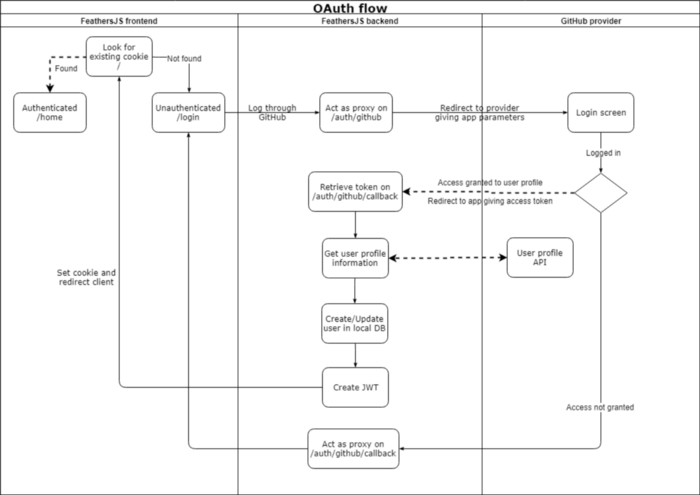
\includegraphics[width=0.80\textwidth]{img/14.png}
\caption{
Funcionamiento de Open Authorization en FeathersJS
Fuente: (Clusters, 2019)}
\label{figure:oAuth}
\end{figure}

\begin{figure}[H]
\centering
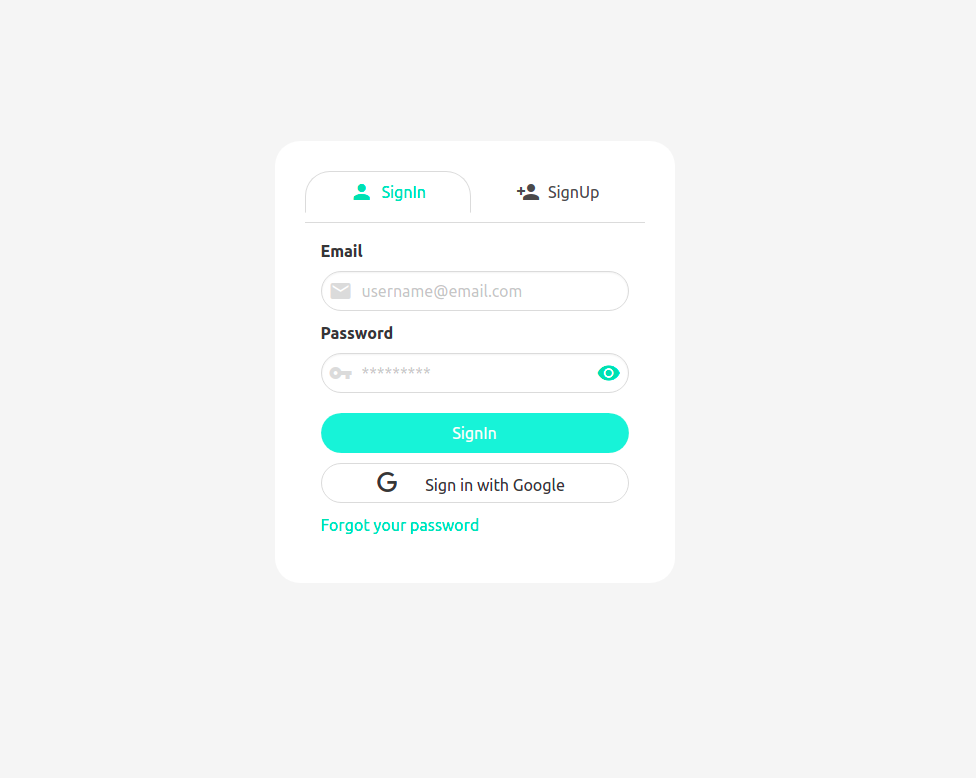
\includegraphics[width=0.80\textwidth]{img/15.png}
\caption{
Inicio de Sesión de la Plataforma
Fuente: Propia}
\label{figure:login}
\end{figure}

\subsection{Autenticación Manual}

Para la implementación manual del proceso de registro, se hizo uso de un proceso de confirmación a través de correo electrónico, como se muestra en la Figura \ref{figure:signup}:


\begin{figure}[H]
\centering
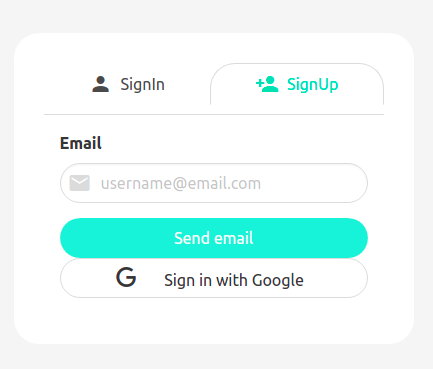
\includegraphics[width=0.60\textwidth]{img/16.png}
\caption{Registro de usuarios. Fuente: Propia}
\label{figure:signup}
\end{figure}


\begin{figure}[H]
\centering
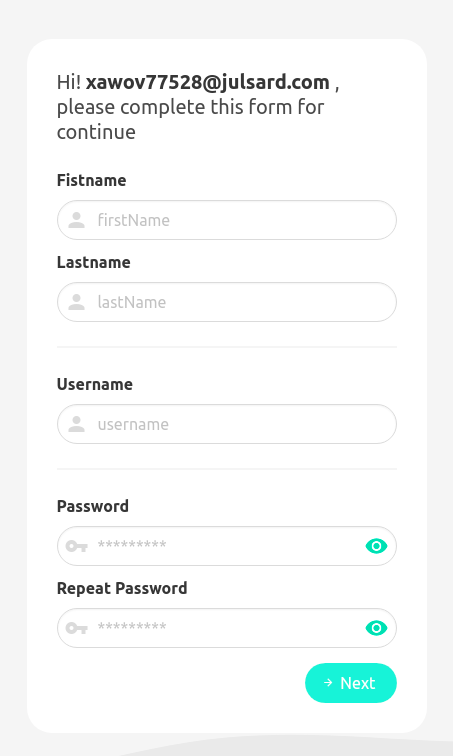
\includegraphics[width=0.60\textwidth]{img/17.png}
\caption{
Formulario Inicial de Usuario. Fuente: Propia}
\label{figure:initialForm}
\end{figure}

En dicho formulario se coloca la información mínima necesario para dar inicio al usuario dentro del sistema. Al ingresar estos datos, ya se encuentra posteriormente en la Vista Inicial, como se aprecia en la Figura \ref{figure:homeView}:

\begin{figure}[H]
\centering
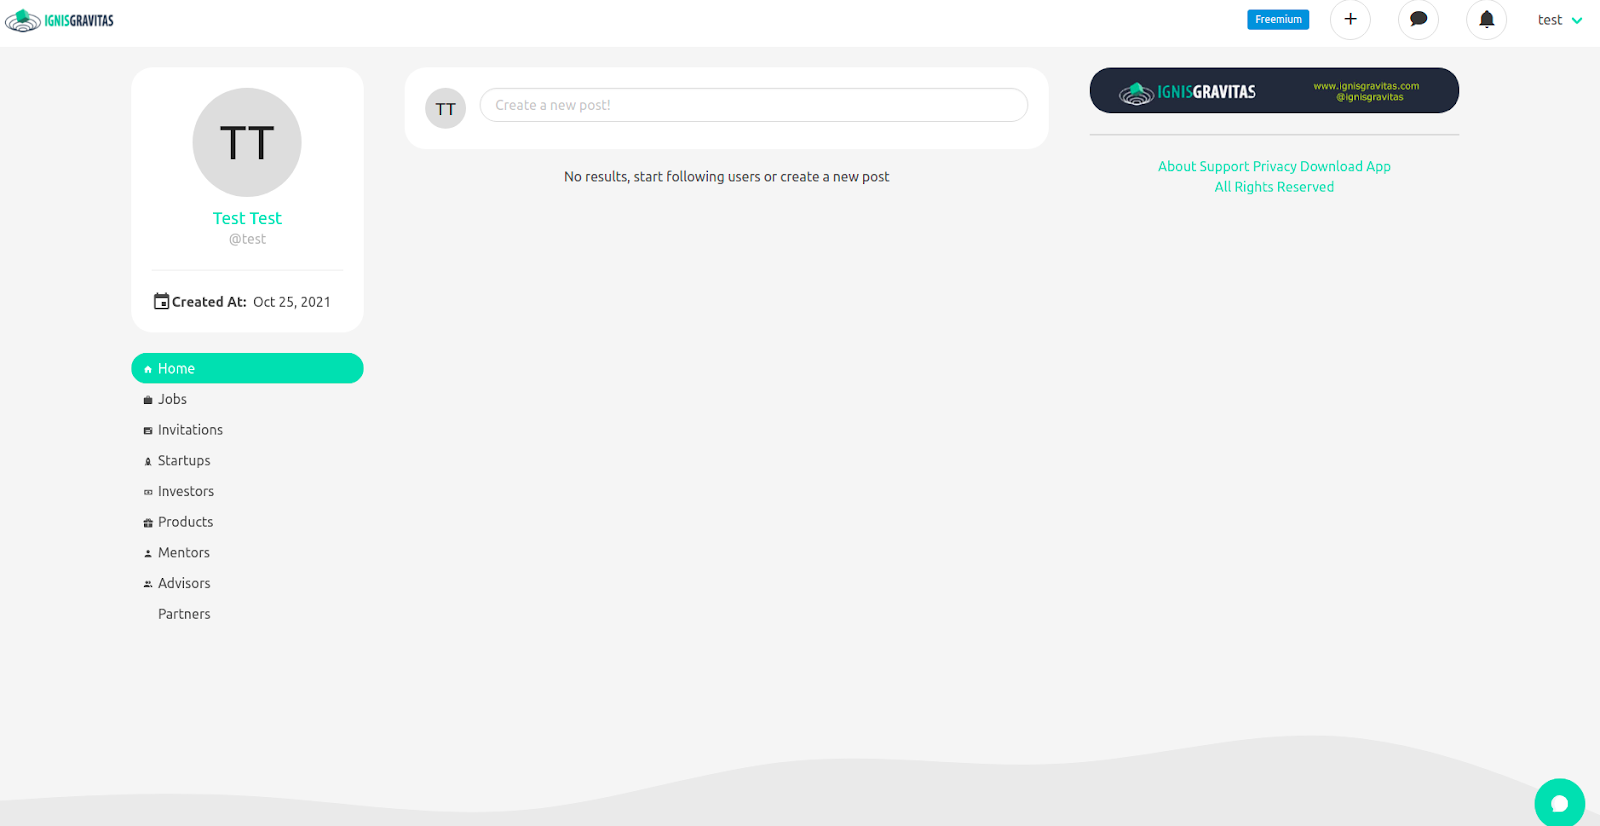
\includegraphics[width=0.60\textwidth]{img/18.png}
\caption{Vista inicial de la plataforma Gravedad. Fuente: Propia}
\label{figure:homeView}
\end{figure}

\section{Vista Interna de la Plataforma}

En esta vista se pueden apreciar las opciones para acceder a las distintas vistas y funcionalidades.

\subsection{Menú General}

Desde la Vista Inicial, se pueden acceder a las distintas opciones de la plataforma:

\begin{figure}[H]
\centering
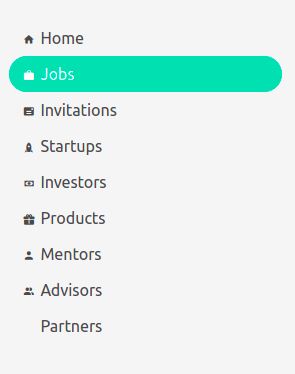
\includegraphics[width=0.60\textwidth]{img/49.png}
\caption{Pila de Opciones de la Plataforma Gravitas. Fuente: Propia}
\label{figure:usersWorkSPref2}
\end{figure}


\begin{figure}[H]
\centering
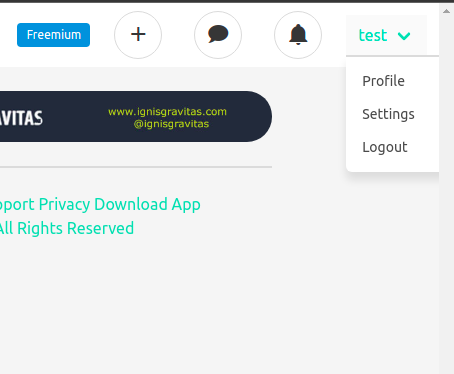
\includegraphics[width=0.60\textwidth]{img/19.png}
\caption{Botón desplegable de la barra de navegación superior.
Fuente: Propia}
\label{figure:dropdown}
\end{figure}

Al acceder a la opción para ver el Perfil de Usuario (Profile), se accede a la vista básica del usuario actual.

\subsection{Usuarios}

Si accedemos a la Vista de Edición de Usuarios, podemos contemplar los siguientes elementos:

\begin{figure}[H]
\centering
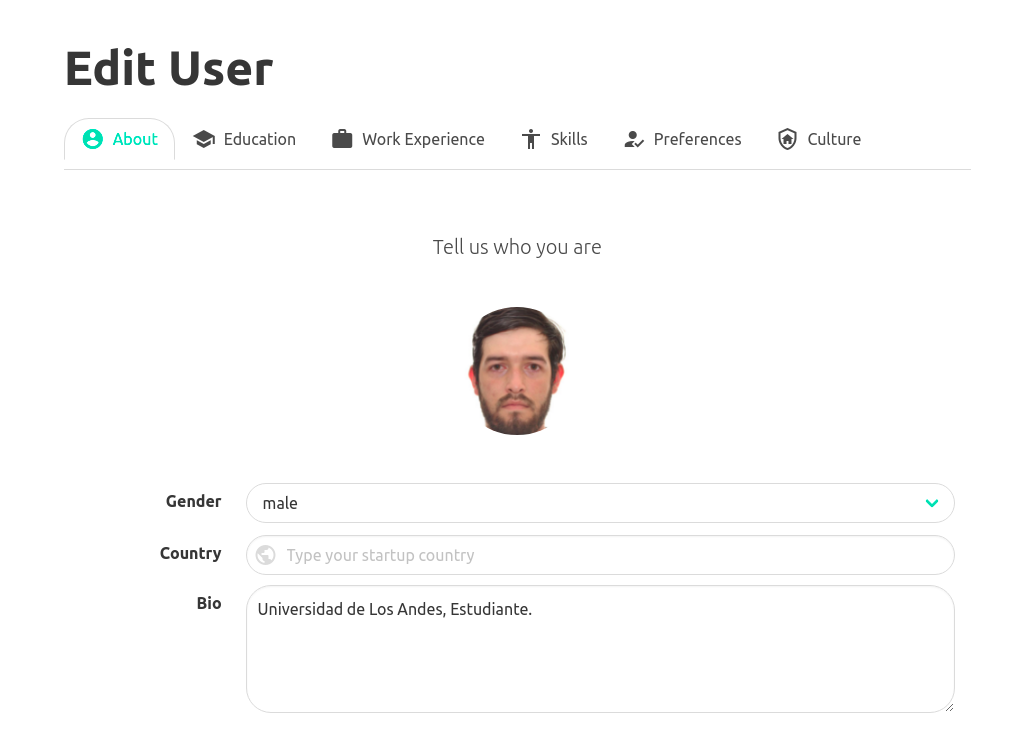
\includegraphics[width=0.60\textwidth]{img/20.png}
\caption{Primera Impresión de la Vista de Usuarios. Fuente: Propia}
\label{figure:usersView}
\end{figure}

En ella podemos ver las seis opciones referentes a la Información General del Usuario, su Educación, Experiencia Laboral, Habilidades, Preferencias como trabajador y su Cultura Individual.

\subsubsection{Información General}

En términos de la Información General, además de la selección estándar de fotografía de perfil, género, país y biografía, se plantea al usuario la selección de otra serie de opciones asociadas a las posiciones que tuvo el usuario previamente en términos laborales, así como la experiencia que posee, los roles preferidos y los roles primarios. Estos dos últimos selectores poseen una serie de opciones precargadas que le permitirán al usuario elegir su rol particular dentro de un conjunto de opciones limitado. Así mismo, se brinda la opción al usuario de introducir información relacionada con sus redes sociales y sitio web personal.

\begin{figure}[H]
\centering
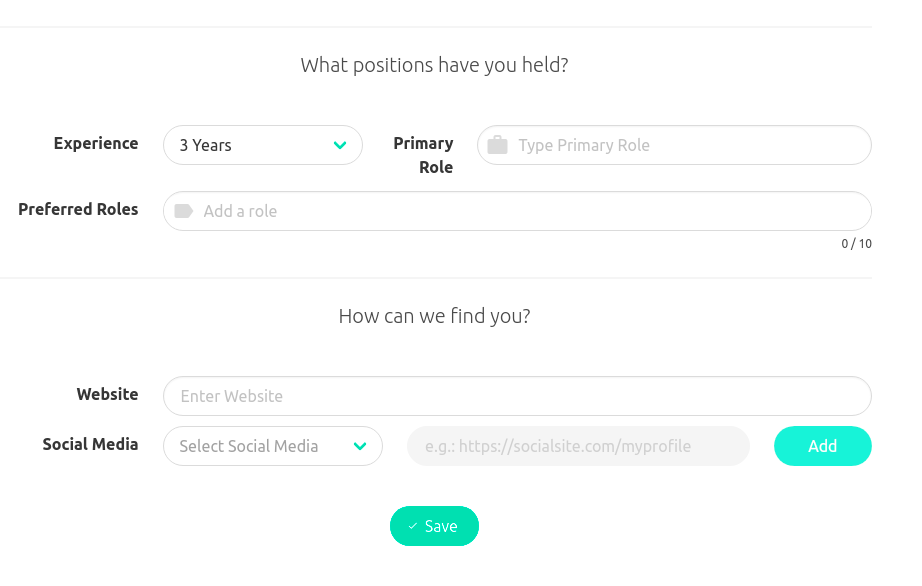
\includegraphics[width=0.60\textwidth]{img/21.png}
\caption{Información General del Perfil de Usuario. Fuente: Propia}
\label{figure:userGeneralInfo}
\end{figure}

\subsubsection{Educación}

\begin{figure}[H]
\centering
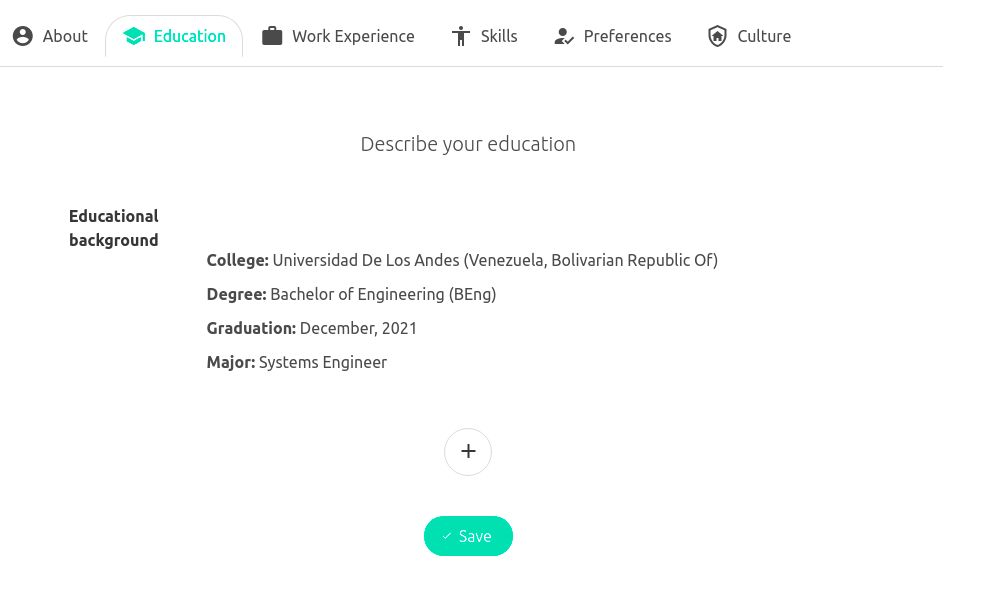
\includegraphics[width=0.60\textwidth]{img/22.png}
\caption{Sección de Educación en el Perfil de Usuario. Fuente: Propia}
\label{figure:usersEducation}
\end{figure}

En el plano de Educación, se desarrolló una lista dinámica a la cual el usuario puede agregar su experiencia académica a través del llenado de un formulario dentro de un modal. Este modal contiene información a introducir tal como: universidad a la que asistió para la titulación, fecha de graduación, grado obtenido y título obtenido.

\begin{figure}[H]
\centering
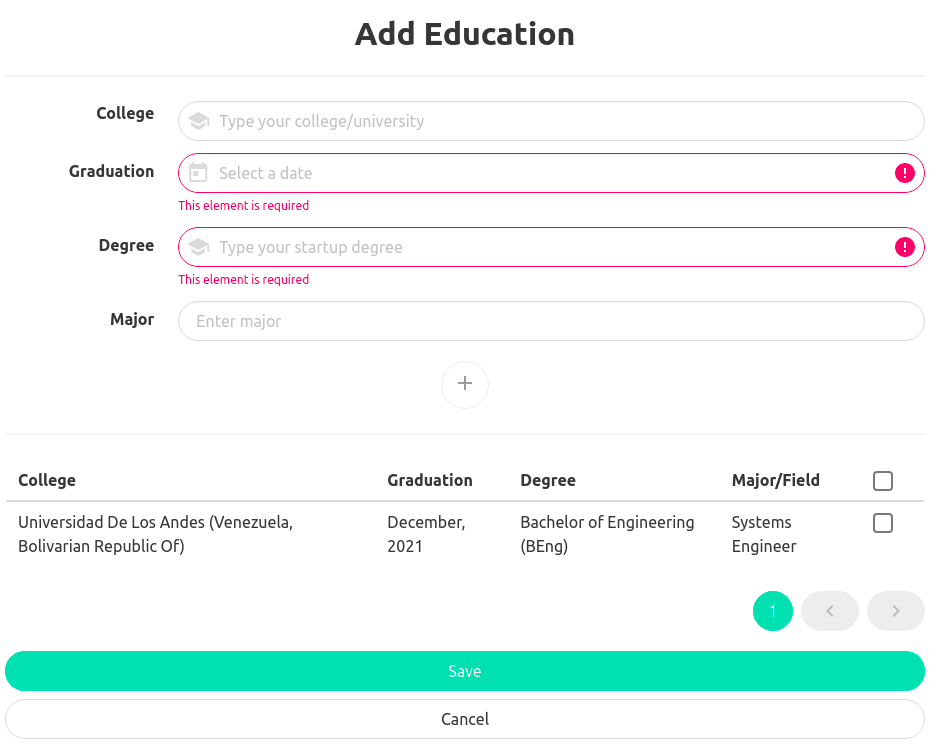
\includegraphics[width=0.60\textwidth]{img/23.png}
\caption{Formulario para añadir nueva experiencia académica. Fuente: Propia}
\label{figure:usersAcademy}
\end{figure}

\begin{figure}[H]
\centering
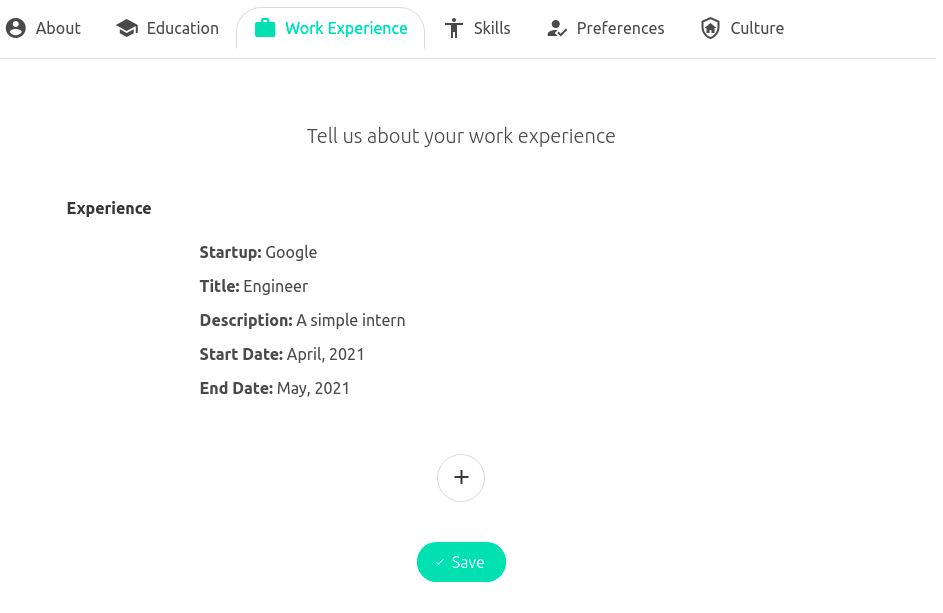
\includegraphics[width=0.60\textwidth]{img/24.png}
\caption{Sección de Experiencia Laboral. Fuente: Propia}
\label{figure:usersWork}
\end{figure}


\subsubsection{Experiencia Laboral}

En el plano laboral, al igual que en el de educación, se hizo uso de una lista dinámica para mostrar la experiencia académica del usuario. El modal que contiene el formulario solicita que se introduzca información referente a la compañía donde trabaja (o trabajó) el usuario, el cargo que ocupó allí, el inicio y final (si aplica) de su prestación de servicios y finalmente una descripción del trabajo realizado.

\begin{figure}[H]
\centering
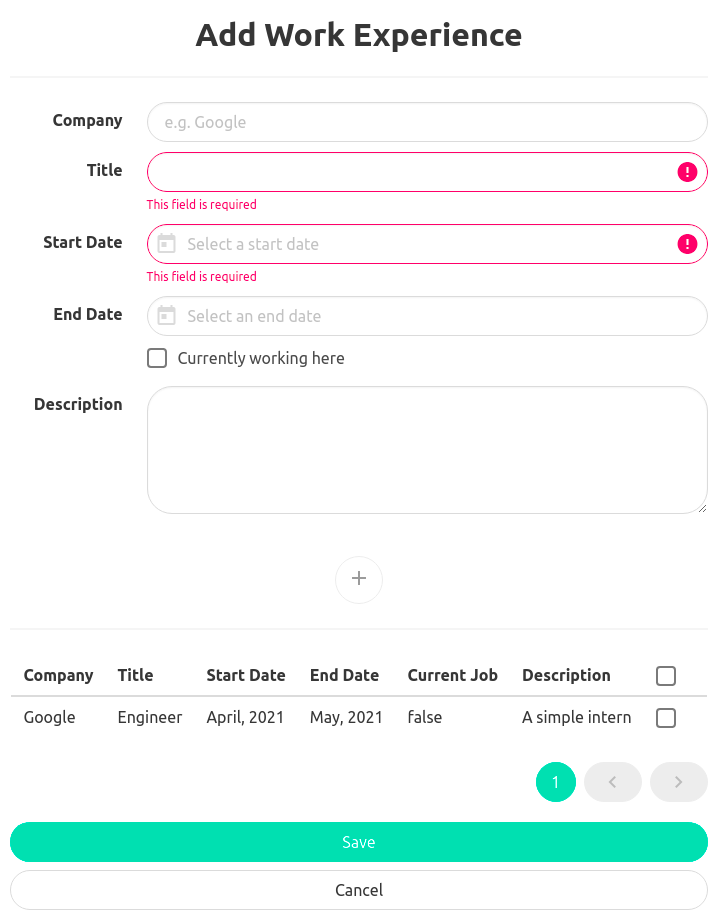
\includegraphics[width=0.60\textwidth]{img/25.png}
\caption{Formulario de Experiencia Laboral. Fuente: Propia}
\label{figure:usersWorkForm}
\end{figure}

\subsubsection{Habilidades Laborales}

Con respecto a las Habilidades Laborales del Usuario, se permite al usuario introducir habilidades dentro de una lista precargada, así como una breve descripción de sus logros y la posibilidad de cargar el currículum.

\begin{figure}[H]
\centering
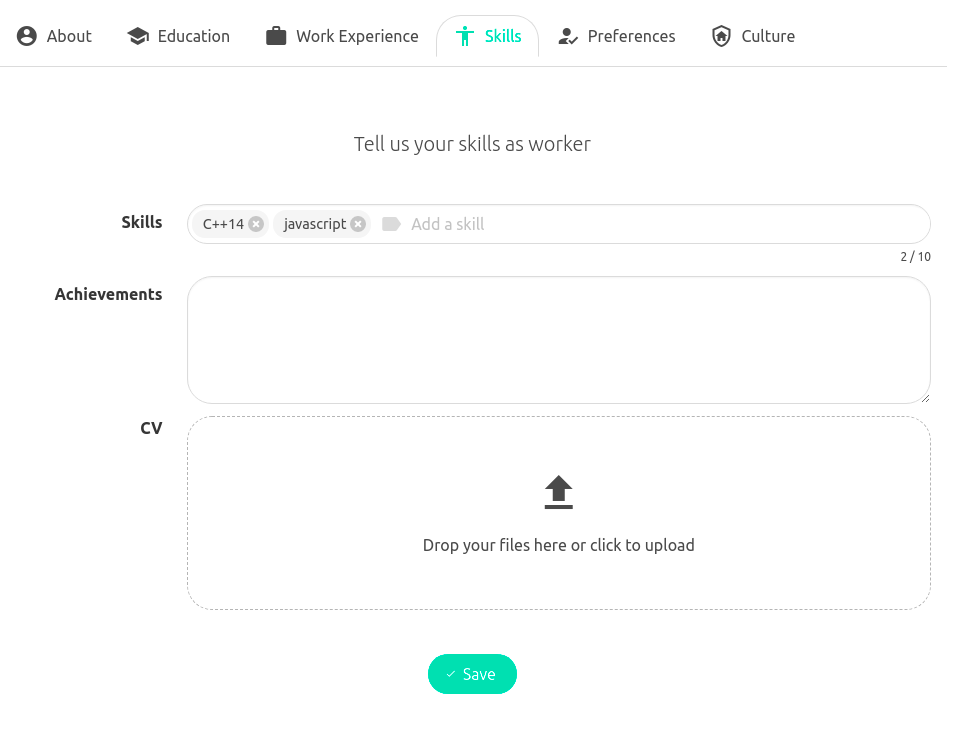
\includegraphics[width=0.60\textwidth]{img/26.png}
\caption{Especificación de Habilidades Laborales. Fuente: Propia}
\label{figure:usersWorkSkills}
\end{figure}

\subsubsection{Preferencias Laborales}

Respecto a las preferencias laborales, la plataforma busca entender los gustos del trabajador y de cómo se siente cómodo trabajando, tanto en su ambiente actual como en términos de salario.

\begin{figure}[H]
\centering
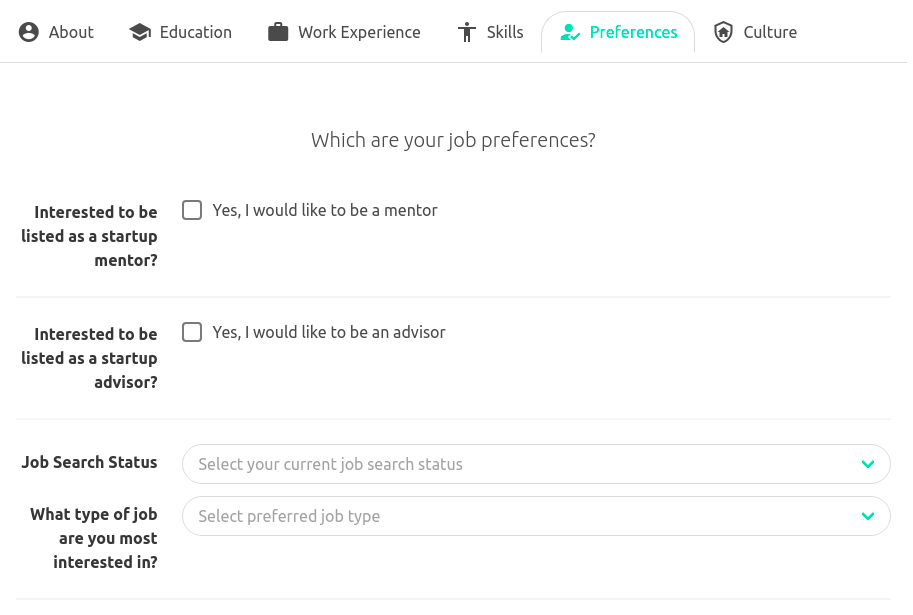
\includegraphics[width=0.60\textwidth]{img/27.png}
\caption{Preferencias Laborales I. Fuente: Propia}
\label{figure:usersWorkSPref1}
\end{figure}

\begin{figure}[H]
\centering
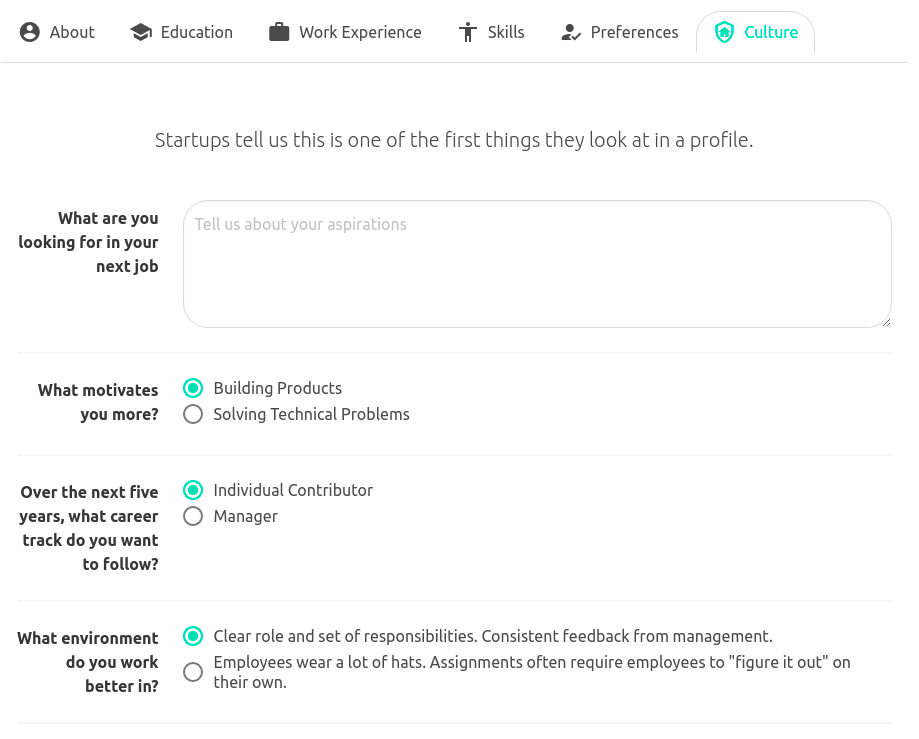
\includegraphics[width=0.60\textwidth]{img/28.png}
\caption{Preferencias Laborales II. Fuente: Propia}
\label{figure:usersWorkSPref2}
\end{figure}

\subsubsection{Cultura Laboral}

Dentro de las opciones para definir las opciones para definir la cultura del usuario, se destacan una serie de preguntas asociadas a las emociones que evoca el mismo como trabajador, por ejemplo la motivación interna del usuario, la proyección a largo plazo y una parametrización en términos de la cultura de la empresa a la que desea aspirar. Esto con el objetivo de encontrar el empleo ideal para este usuario en un futuro sistema de recomendaciones.

\begin{figure}[H]
\centering
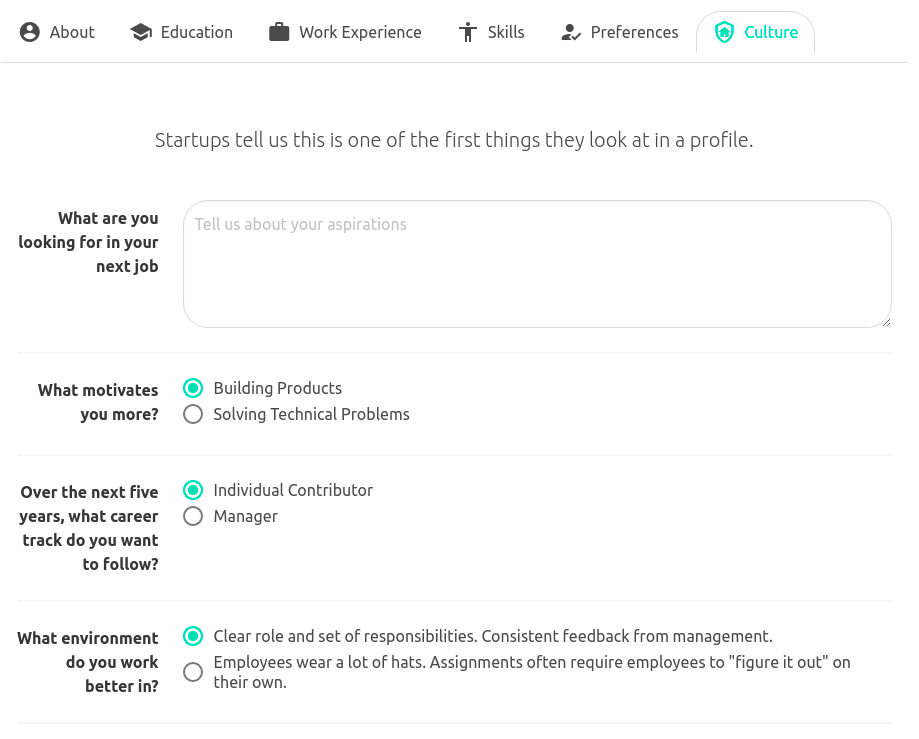
\includegraphics[width=0.60\textwidth]{img/29.png}
\caption{Cultura Laboral del Usuario I. Fuente: Propia}
\label{figure:usersCulture1}
\end{figure}


\begin{figure}[H]
\centering
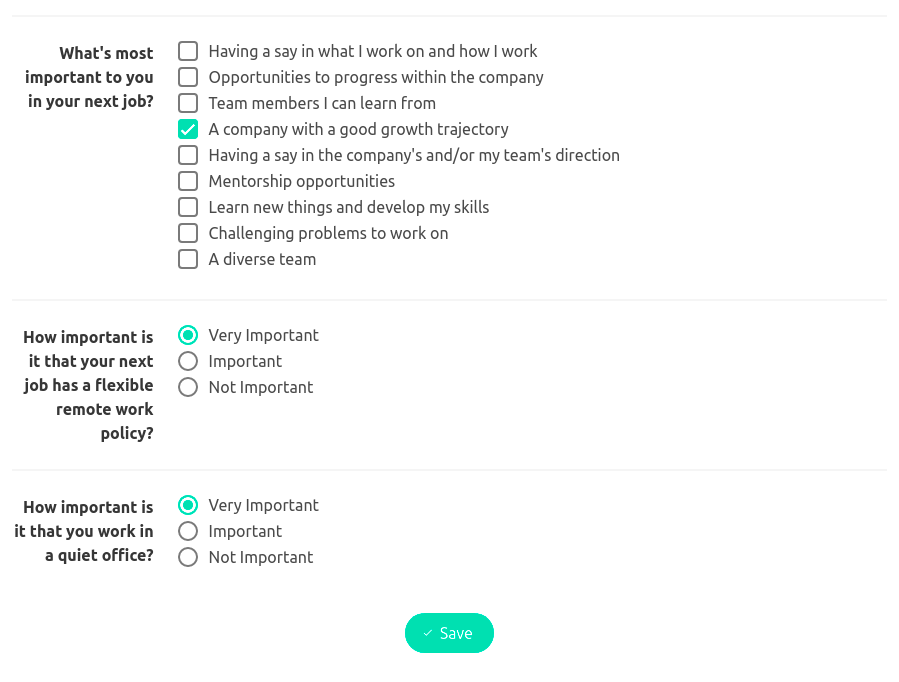
\includegraphics[width=0.60\textwidth]{img/30.png}
\caption{Cultura Laboral del Usuario II. Fuente: Propia}
\label{figure:usersCulture2}
\end{figure}

Finalmente, el perfil de usuario tiene la siguiente forma:

\begin{figure}[H]
\centering
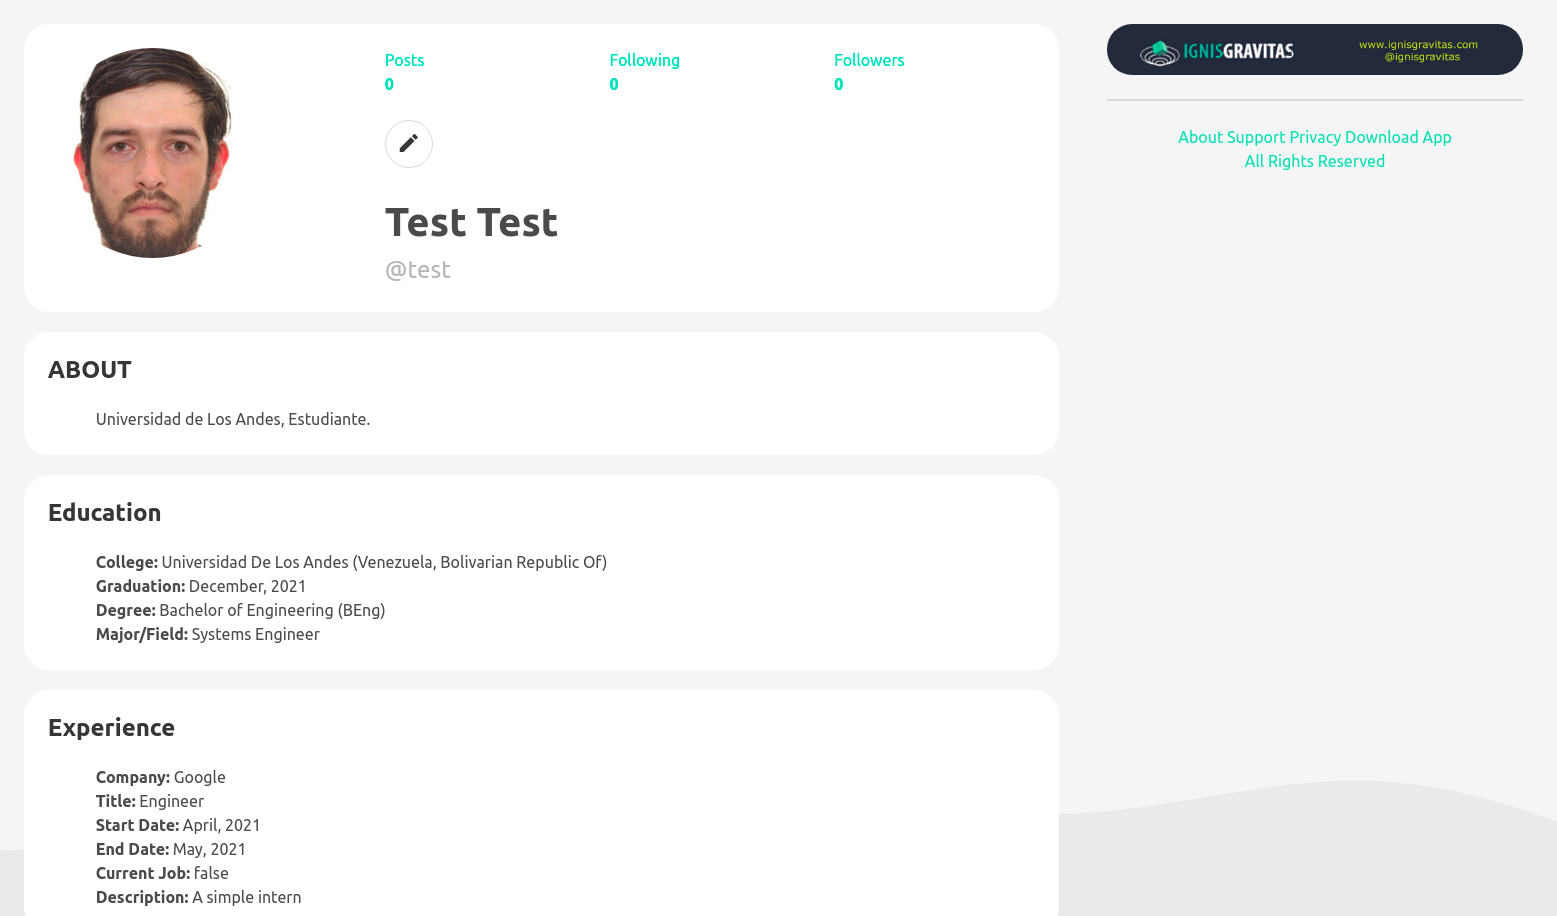
\includegraphics[width=0.60\textwidth]{img/31.png}
\caption{Perfil de usuario. Fuente: Propia}
\label{figure:usersProfile}
\end{figure}

\subsection{Cuenta}

La vista de configuración de la cuenta, por su parte, únicamente tiene información básica, tal como el nombre y apellido, dirección correo electrónico, nombre de usuario y cambio de contraseña. Las demás opciones asociadas a privacidad, preferencias de cuenta e integraciones no se encuentran disponibles.

\begin{figure}[H]
\centering
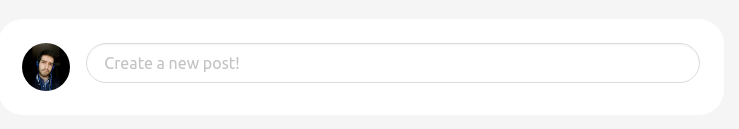
\includegraphics[width=0.60\textwidth]{img/32.png}
\caption{Menú de Configuración de Cuenta. Fuente: Propia}
\label{figure:accountMenu}
\end{figure}

\subsection{Publicaciones}

Si deseamos crear una publicación, solo hace falta hacer click sobre la entrada de texto de “Crear un nuevo Post” en la sección central del menú inicial.

\begin{figure}[H]
\centering
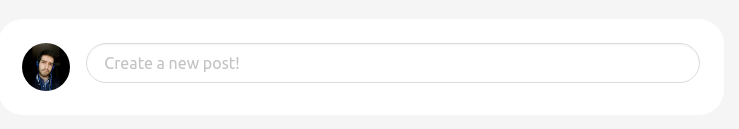
\includegraphics[width=0.60\textwidth]{img/33.png}
\caption{Espacio de creación de Posts. Fuente: Propia}
\label{figure:postsCreation}
\end{figure}


Al realizar dicha acción, se va a desplegar un modal que muestra nuevamente una entrada de texto y otra serie de campos interactivos que permiten la inserción de imágenes y archivos. Allí se puede describir el contenido textual de la publicación, así como quién está realizando la publicación (si es una startup, un producto o un usuario) y las imágenes y contenido multimedia asociado.

\begin{figure}[H]
\centering
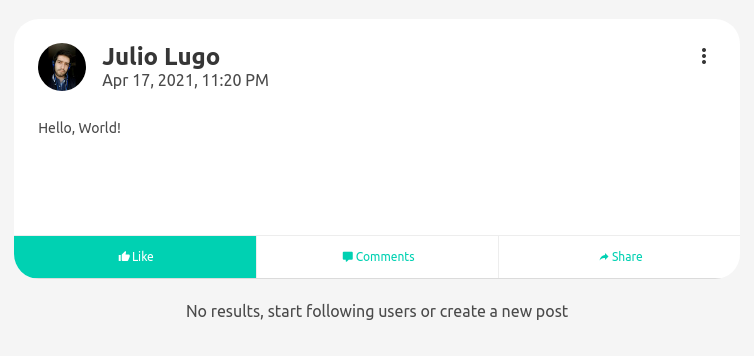
\includegraphics[width=0.60\textwidth]{img/34.png}
\caption{Formulario para la creación de Publicaciones. Fuente: Propia}
\label{figure:postsCreationForm}
\end{figure}


Al crearse una publicación, la misma es listada en tiempo real en la vista principal. La publicación también puede ser editada o eliminada dentro del menú en la parte superior de la publicación. Todas las publicaciones, al ser creadas, incluyen las siguientes funcionalidades:
La función de interacción “Me gusta”, para indicar apoyo a una publicación.
La función de comentar, que permite a los usuarios seguidores de otro usuario, startup o producto, emitir opiniones. También pueden editar o eliminar dichos comenarios.
La función de compartir publicación, para que dicha publicación sea listada también para los usuarios seguidores de cualquiera que comparta la publicación y no únicamente de quien la creó.

\begin{figure}[H]
\centering
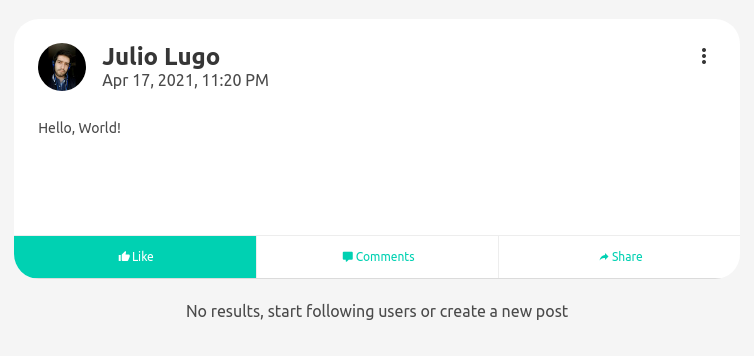
\includegraphics[width=0.60\textwidth]{img/35.png}
\caption{
Publicación listada en la Vista Inicial. Fuente: Propia}
\label{figure:homeViewPost}
\end{figure}

Si el usuario clickea sobre la fecha y hora de la publicación, podrá ingresar a una vista dedicada donde únicamente tendrá la publicación presente. Esta vista dedicada puede ser compartida a través de un link, por si se desea llevar a un lugar externo a la plataforma. Todo usuario puede crear nuevos perfiles, tanto para una Startup como para un Producto.  Asímismo, se puede solicitar la posibilidad de ser inversor o de convertirse en un Aliado para que, manualmente, un desarrollador de Ignis Gravitas incorpore a dicho individuo al listado de inversores o aliados claves previa aprobación de la compañía Ignis Gravitas, Inc.

\begin{figure}[H]
\centering
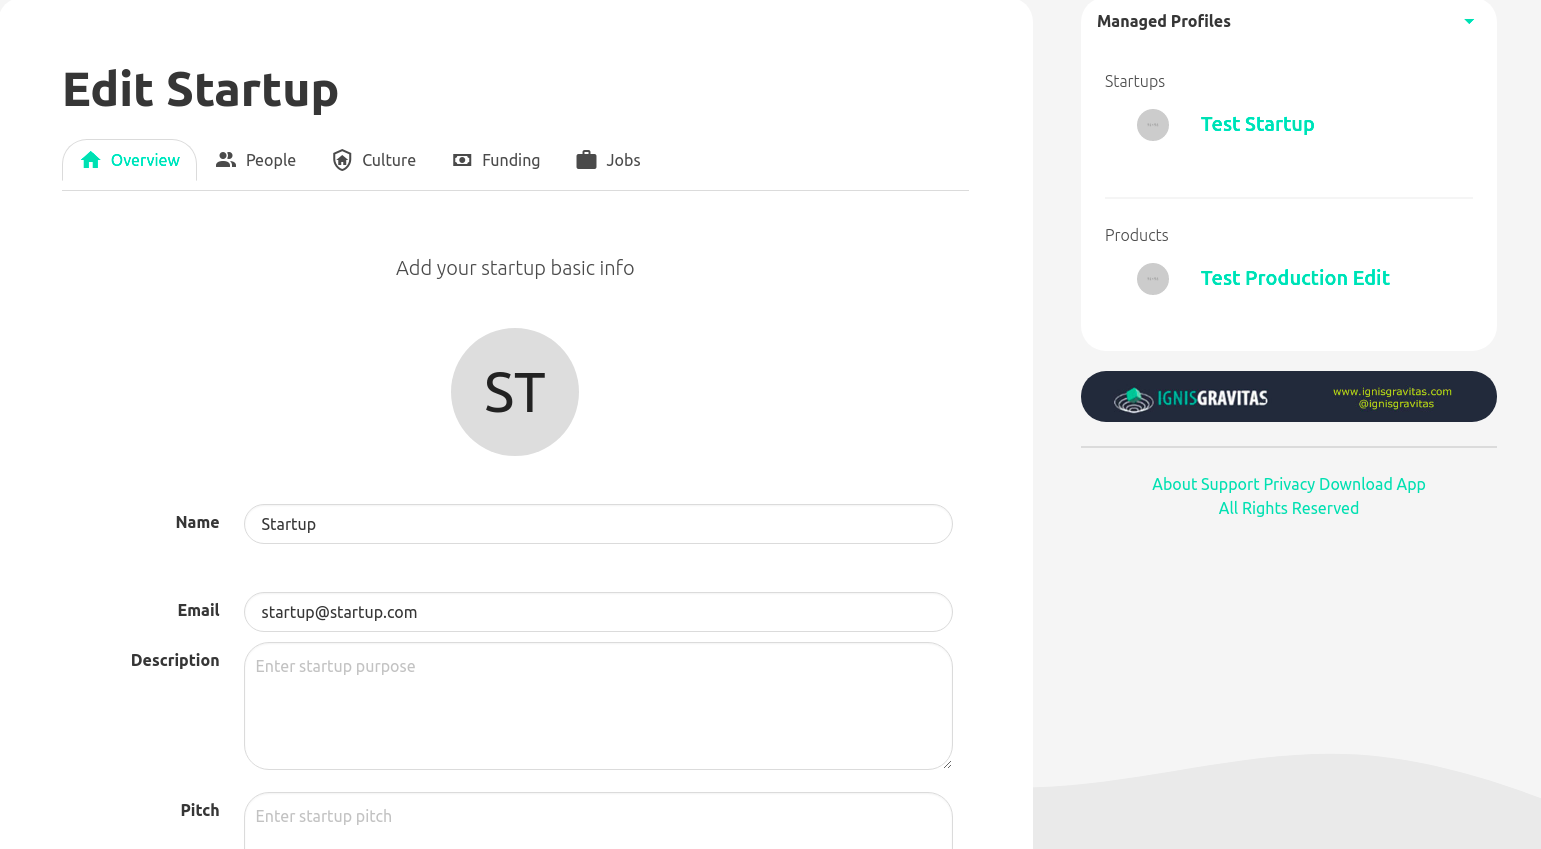
\includegraphics[width=0.60\textwidth]{img/36.png}
\caption{Menú desplegable para la creación de perfiles. Fuente: Propia}
\label{figure:dropdownProfiles}
\end{figure}


\subsection{Startups}	

Al seleccionar Crear Perfil de Startup, dicho usuario accederá a una vista de creación particular que se enfoca únicamente en la vista de las startups. Esta vista contiene una serie de secciones: Resumen, Personas, Cultura, Fondos y Trabajos.

\begin{figure}[H]
\centering
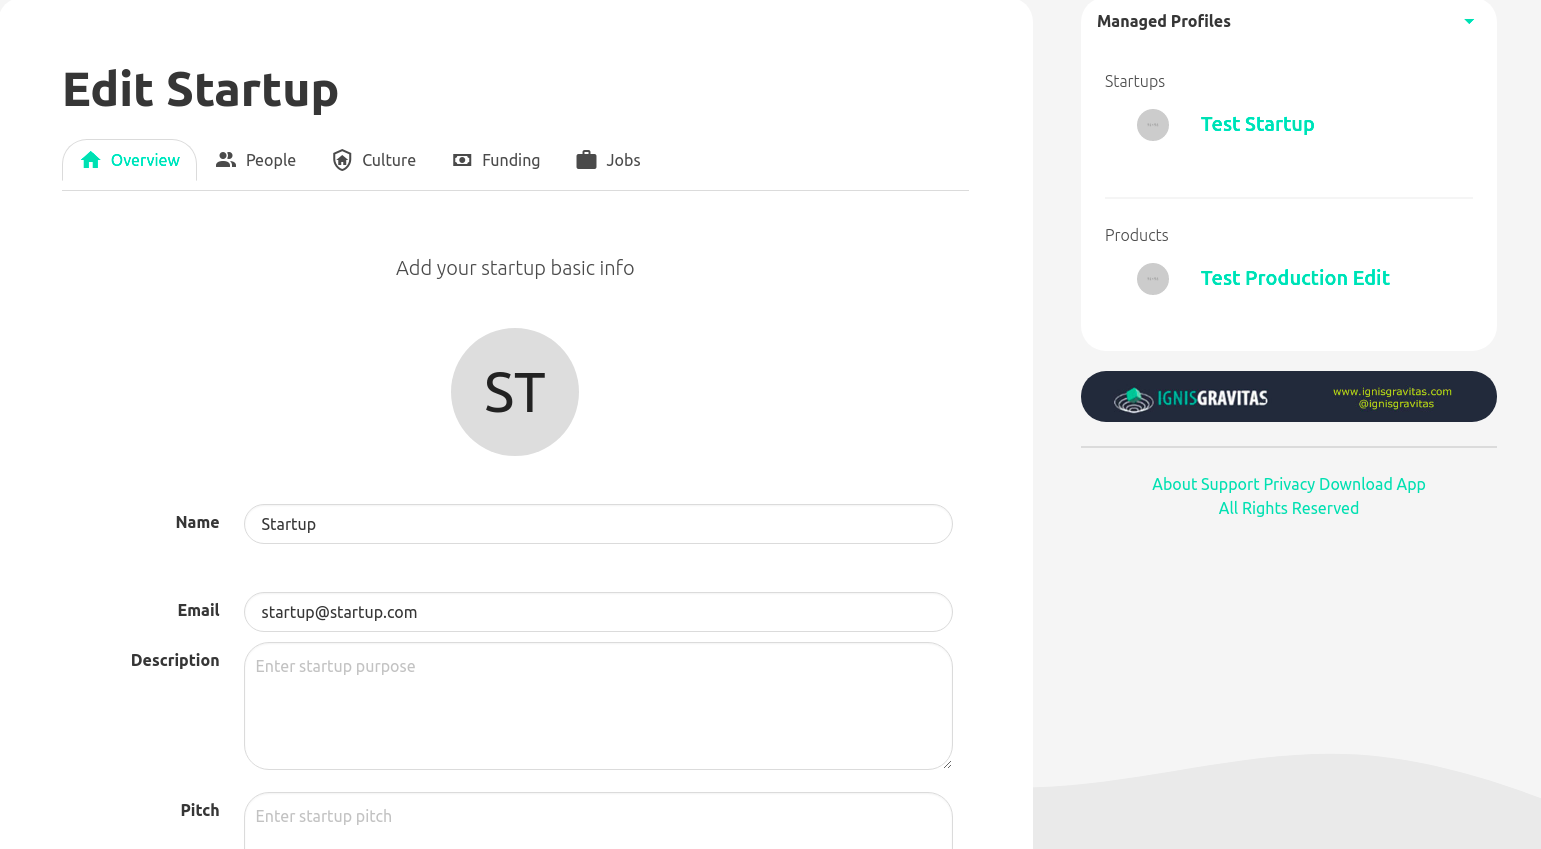
\includegraphics[width=0.60\textwidth]{img/37.png}
\caption{Formulario de Creación de Startups. Fuente: Propia}
\label{figure:startupsCreation}
\end{figure}

\subsubsection{Resumen}

Cada una de estas secciones contiene dentro de sí otra serie de datos de entrada. En la primera sección, se solicita la información básica de la startup, que se engloba en: Nombre de la Startup, dirección de correo electrónico, descripción básica de la startup, discurso de venta de la startup (pitch), país de origen, ciudad de origen, dirección física, dirección del sitio web de la startup, enlaces a las Redes Sociales de la startup, selección de los mercados a los cuales apunta la startup, enlace a un vídeo introductorio de la startup y, finalmente, historias de usuarios satisfechos con el trabajo de la startup.

\begin{figure}[H]
\centering
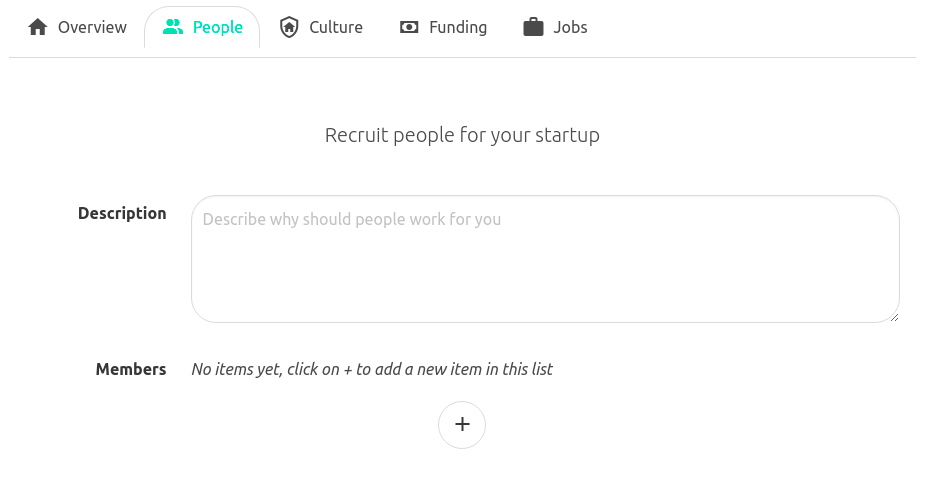
\includegraphics[width=0.60\textwidth]{img/38.png}
\caption{Formulario de Información Básica de la Startup. Fuente: Propia}
\label{figure:startupsBasicInfoForm}
\end{figure}

\subsubsection{Personas}

En la segunda vista, se pueden realizar las adiciones de membresías y hacer una descripción somera de lo que significa el equipo para la startup.

\begin{figure}[H]
\centering
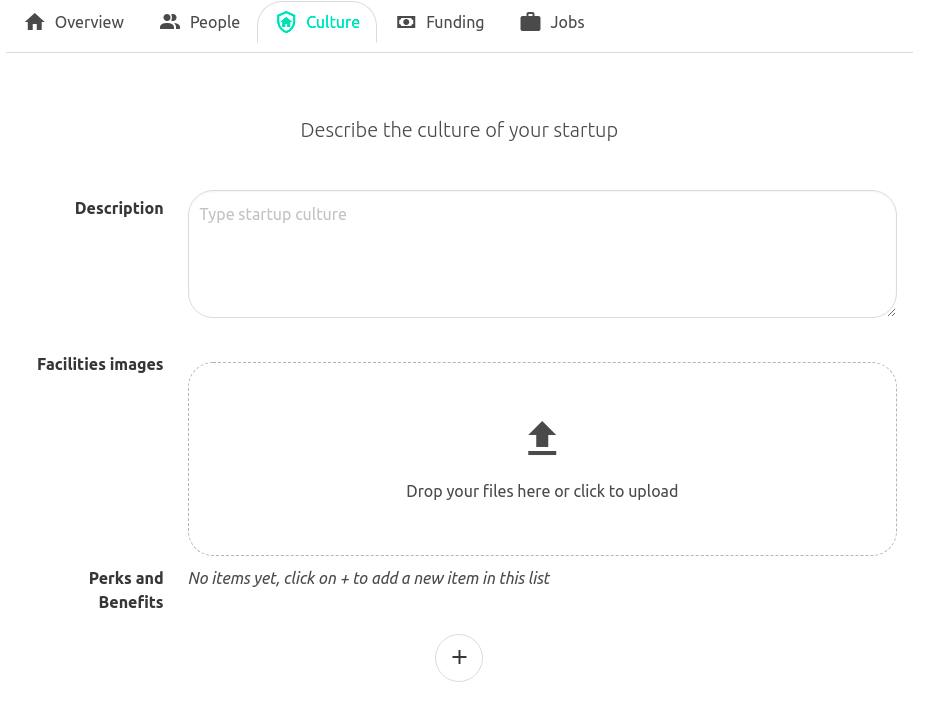
\includegraphics[width=0.60\textwidth]{img/39.png}
\caption{Formulario de la Sección Personas. Fuente: Propia}
\label{figure:startupsPeople}
\end{figure}

Al hacer click en el botón de agregar, se despliega un nuevo formulario que permite invitar nuevos miembros a la Startup. Estos nuevos miembros aparecerán luego en el perfil de la startup.

\begin{figure}[H]
\centering
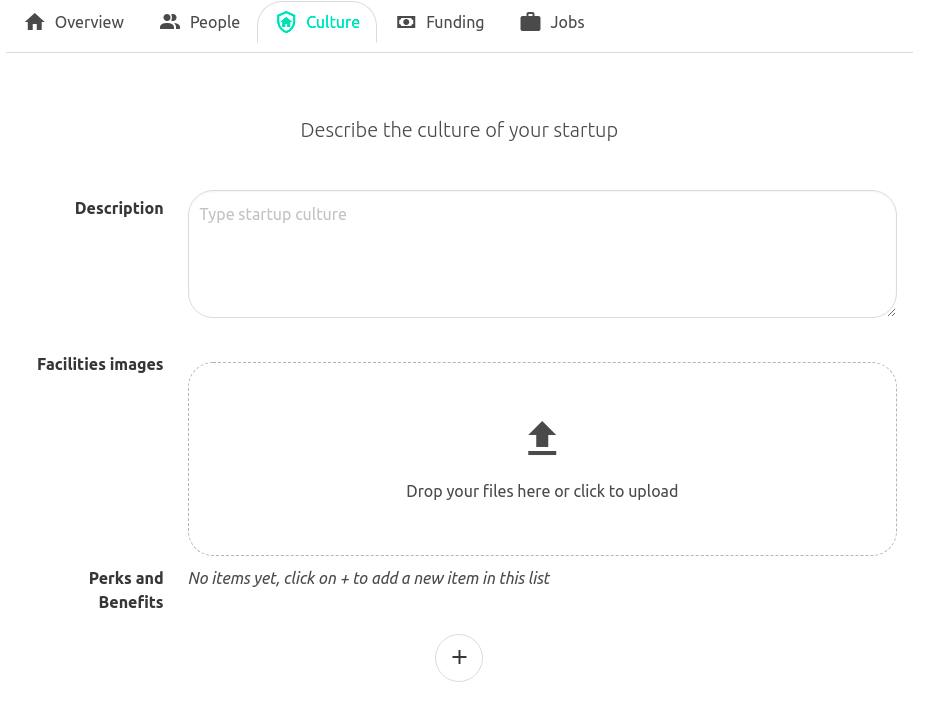
\includegraphics[width=0.60\textwidth]{img/40.png}
\caption{Formulario para añadir un nuevo miembro. Fuente: Propia}
\label{figure:startupsAddMember}
\end{figure}

\subsubsection{Cultura}

En la sección cultura, se añaden nuevas entradas de texto referentes a la descripción cultural de la startup, así como una serie de entrada de archivos para subir imágenes que muestren referencias a la compañía, como sus sitios de trabajo, personal, productos, etc. Además, se pueden agregar los beneficios y ventajas que ofrece la startup a cada uno de sus empleados.

\begin{figure}[H]
\centering
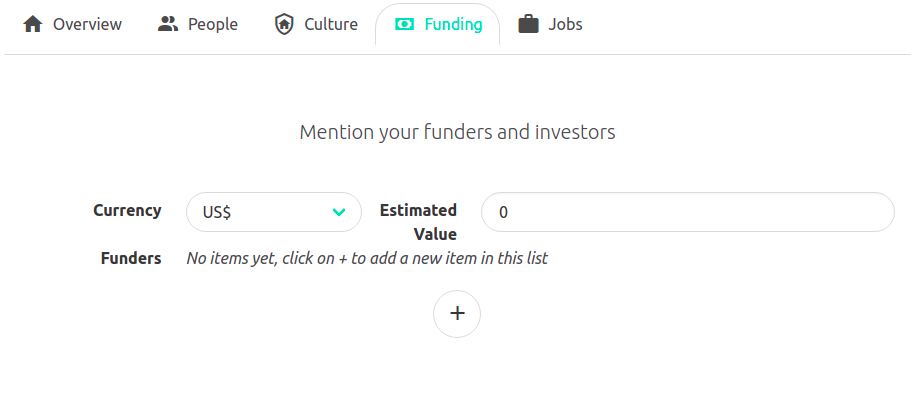
\includegraphics[width=0.60\textwidth]{img/41.png}
\caption{Formulario de la Sección Cultura. Fuente: Propia}
\label{figure:startupsCulture}
\end{figure}


\begin{figure}[H]
\centering
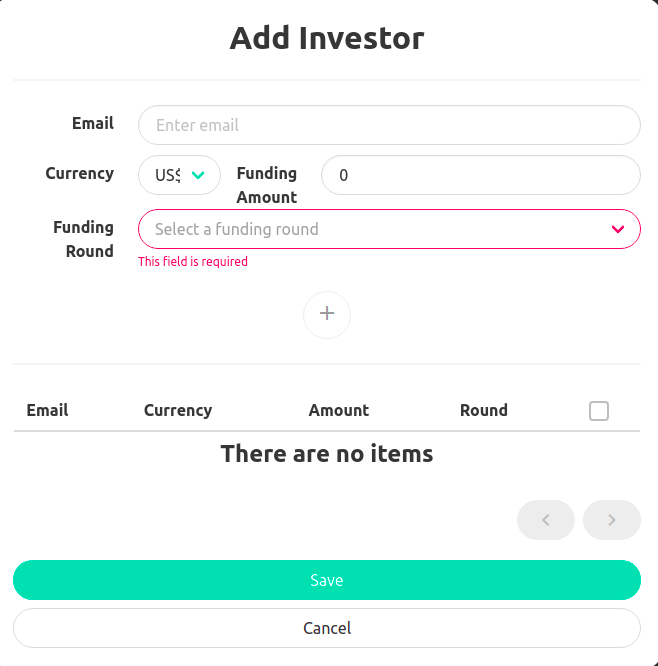
\includegraphics[width=0.60\textwidth]{img/42.png}
\caption{
Añadir un nuevo beneficio. Fuente: Propia}
\label{figure:startupsPerk}
\end{figure}

\subsubsection{Financiamient}

En la sección de Financiamiento, se puede agregar la cantidad de dinero recibida hasta el momento, así como los inversores que han hecho contribuciones a la startup.

\begin{figure}[H]
\centering
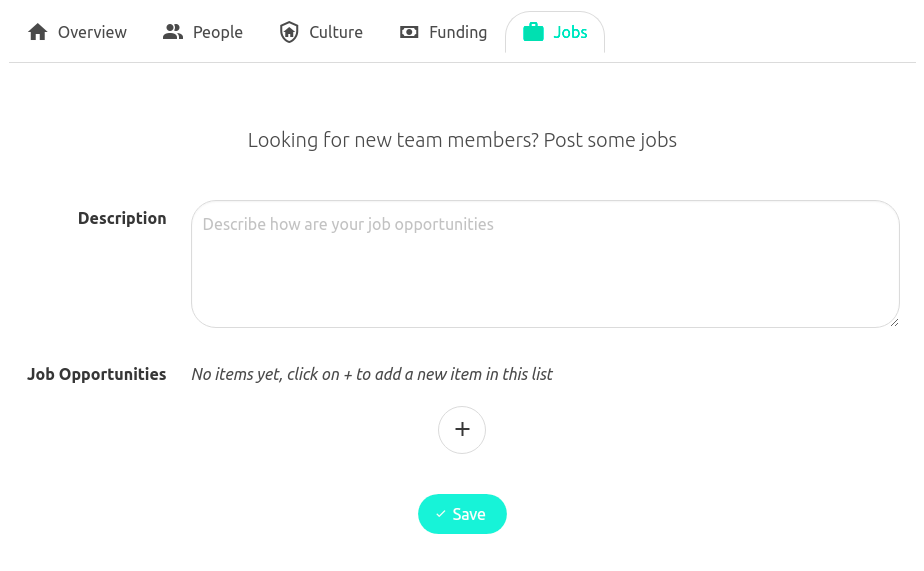
\includegraphics[width=0.60\textwidth]{img/43.png}
\caption{
Entrada de datos de la sección Financiamiento. Fuente: Propia}
\label{figure:startupFunding}
\end{figure}


\begin{figure}[H]
\centering
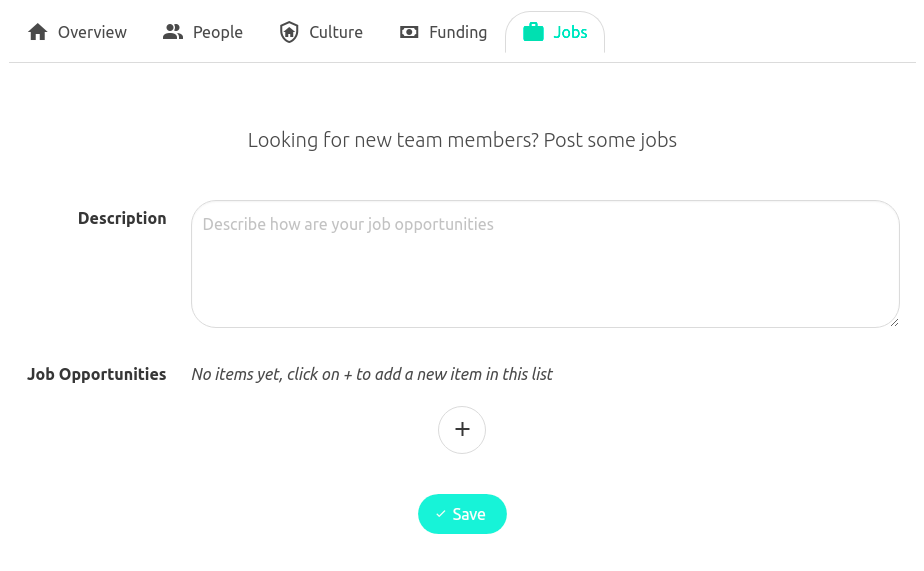
\includegraphics[width=0.60\textwidth]{img/44.png}
\caption{Formulario para añadir un inversor. Fuente: Propia}
\label{figure:startupAddInvestor}
\end{figure}

\subsubsection{Trabajos}

En la sección de trabajos, se puede agregar la descripción general de la startup, así como las oportunidades de trabajo asociadas a la misma.

\begin{figure}[H]
\centering
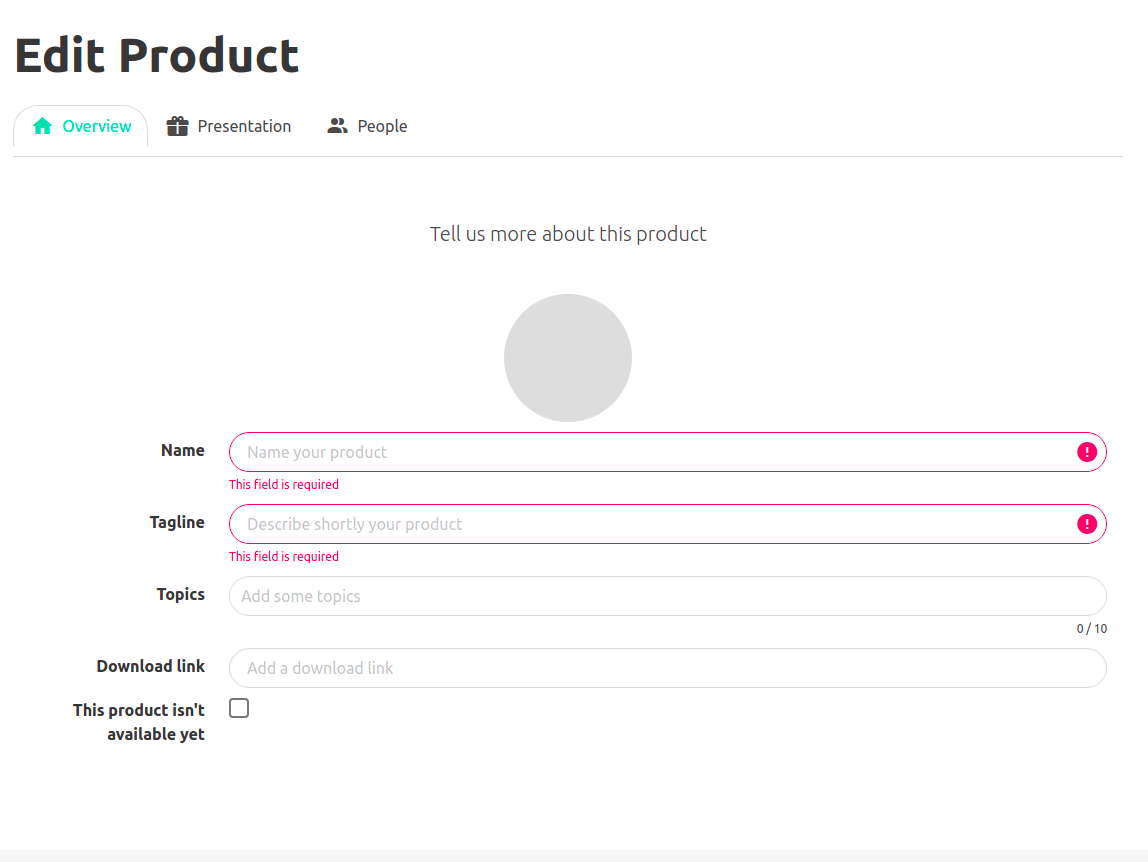
\includegraphics[width=0.60\textwidth]{img/45.png}
\caption{Entrada de datos en la sección Trabajo. Fuente: Propia}
\label{figure:startupWork}
\end{figure}


\begin{figure}[H]
\centering
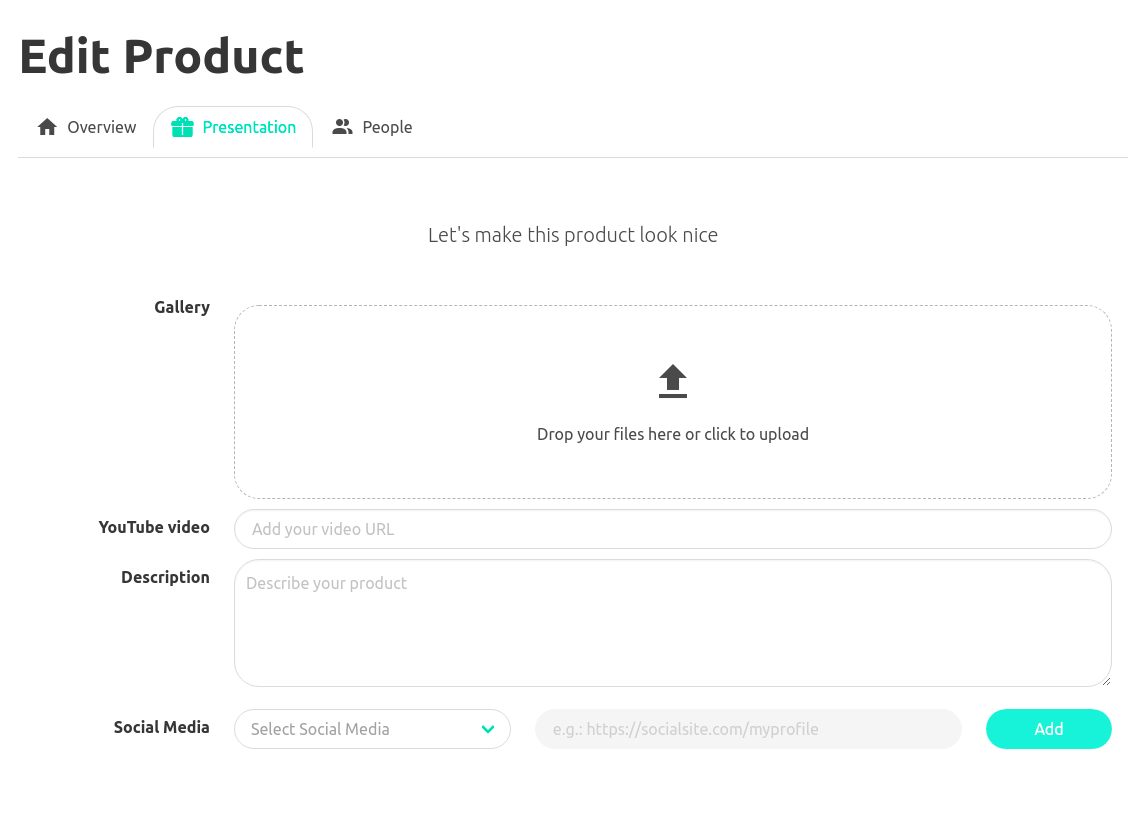
\includegraphics[width=0.60\textwidth]{img/46.png}
\caption{Formulario para propuestas de trabajo. Fuente: Propia}
\label{figure:startupWorkForm}
\end{figure}

\subsection{Productos}

Al buscar crear un producto, se muestran el siguiente formulario:
El mismo, dividido en tres pestañas (“Resumen”, “Presentación” y “Personas”) permite detallar el producto ofertado. Los productos son, en una primera versión, independientes de las startups.

\begin{figure}[H]
\centering
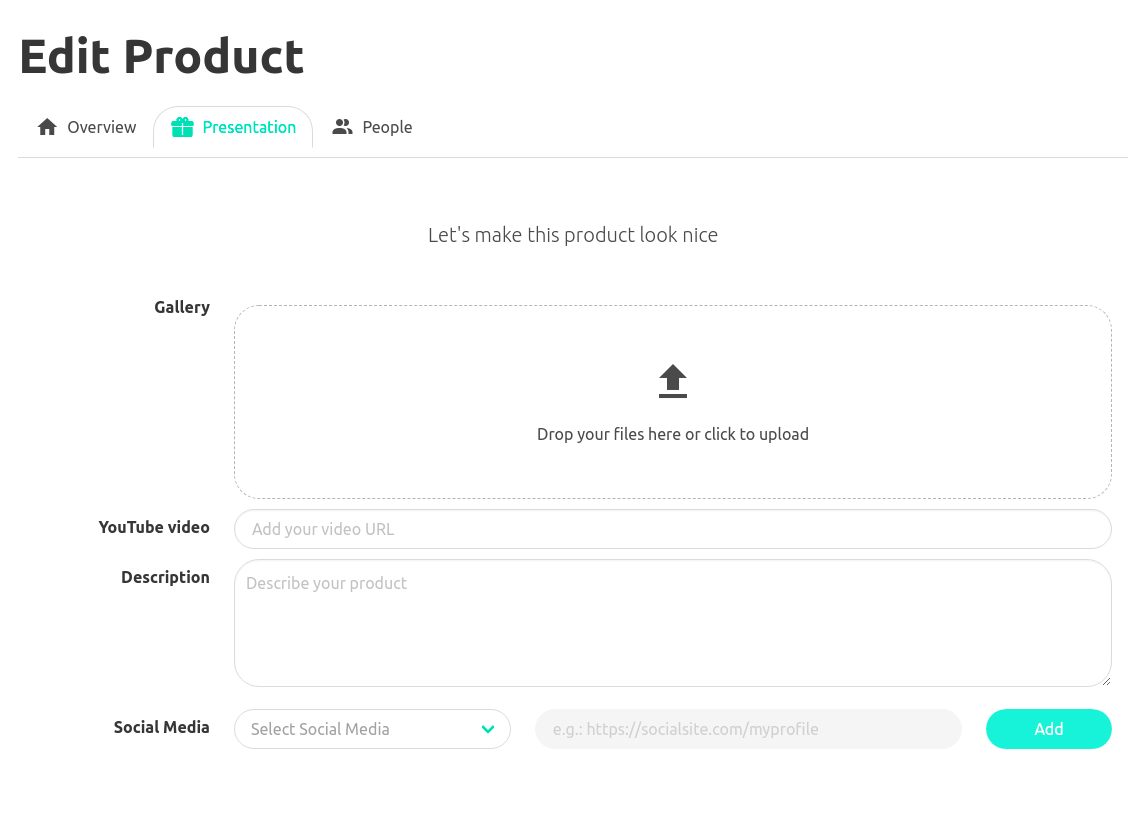
\includegraphics[width=0.60\textwidth]{img/47.png}
\caption{Sección Presentación. Fuente: Propia}
\label{figure:productPresentation}
\end{figure}

\begin{figure}[H]
\centering
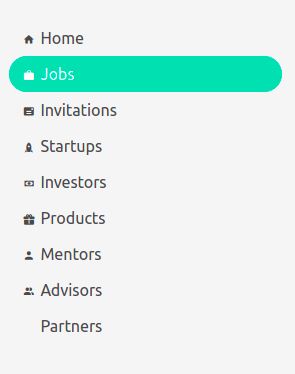
\includegraphics[width=0.60\textwidth]{img/48.png}
\caption{Edición de Productos. Fuente: Propia}
\label{figure:productEdition}
\end{figure}


\subsection{Trabajos}

El listado de trabajos es accesible desde la Pila de Opciones en el menú lateral. La misma posee la siguiente interfaz gráfica:

\begin{figure}[H]
\centering
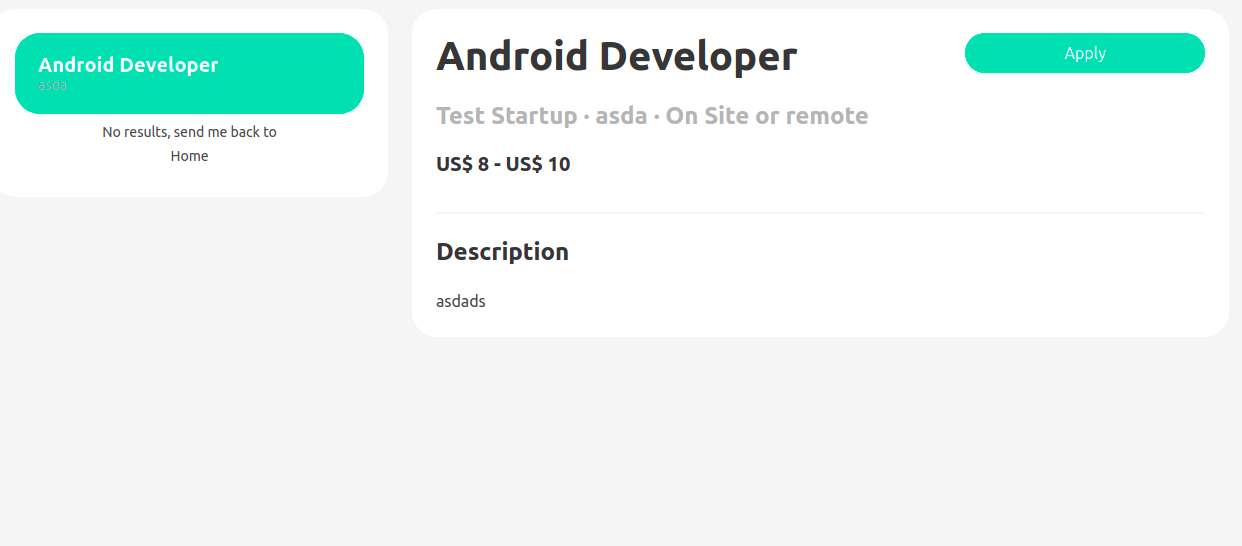
\includegraphics[width=0.60\textwidth]{img/50.png}
\caption{
Vista de Listado de Trabajos. Fuente: Propia}
\label{figure:jobsList}
\end{figure}

Del lado izquierdo, se ven las distintas ofertas de trabajo a las cuales puede aplicar un desarrollador, y a la derecha, una descripción detallada de la misma. Al hacer click sobre “Aplicar”, se muestra el siguiente formulario:


\begin{figure}[H]
\centering
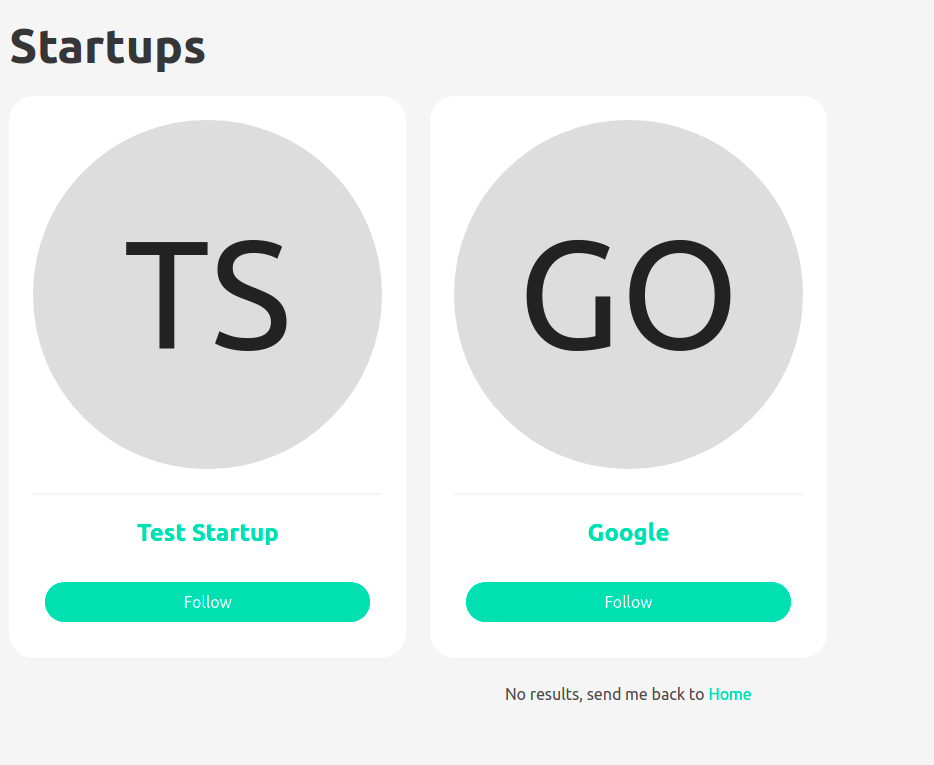
\includegraphics[width=0.60\textwidth]{img/51.png}
\caption{
Formulario de aplicación a propuestas de trabajo. Fuente: Propia}
\label{figure:jobApplicationForm}
\end{figure}

\subsection{Indexación}

\subsubsection{Listado de Startups}

\begin{figure}[H]
\centering
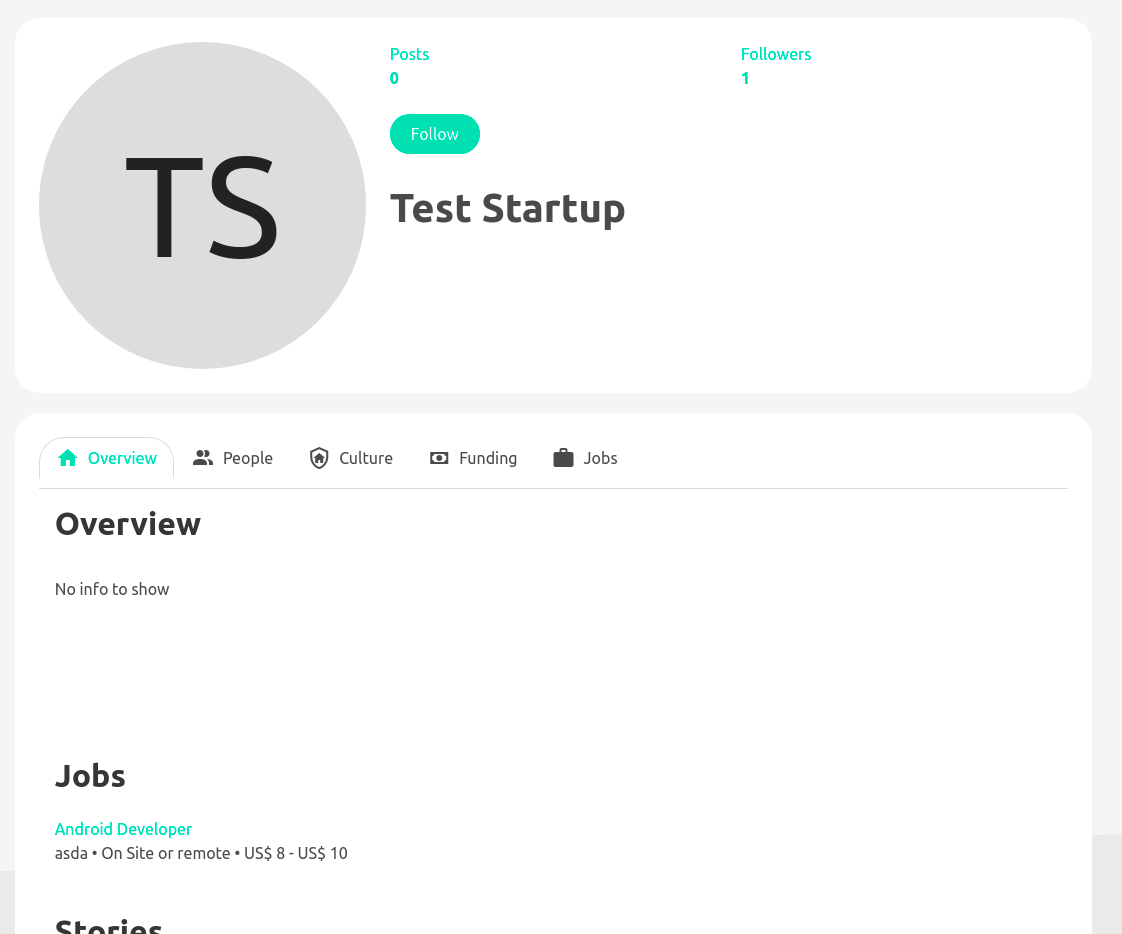
\includegraphics[width=0.60\textwidth]{img/52.png}
\caption{Listado de Startup. Fuente: Propia}
\label{figure:startupList}
\end{figure}

Al acceder al listado de startups, se puede contemplar cada una de las startups creadas por los distintos usuarios, así como aquellas sugeridas durante la selección del empleo previo, como un perfil creado por la comunidad y que no puede ser gestionado hasta no haber sido pedido y su autenticidad verificada.

Cada perfil contiene la información introducida en un principio de manera ordenada, así como los posts que ha publicado previamente:

\begin{figure}[H]
\centering
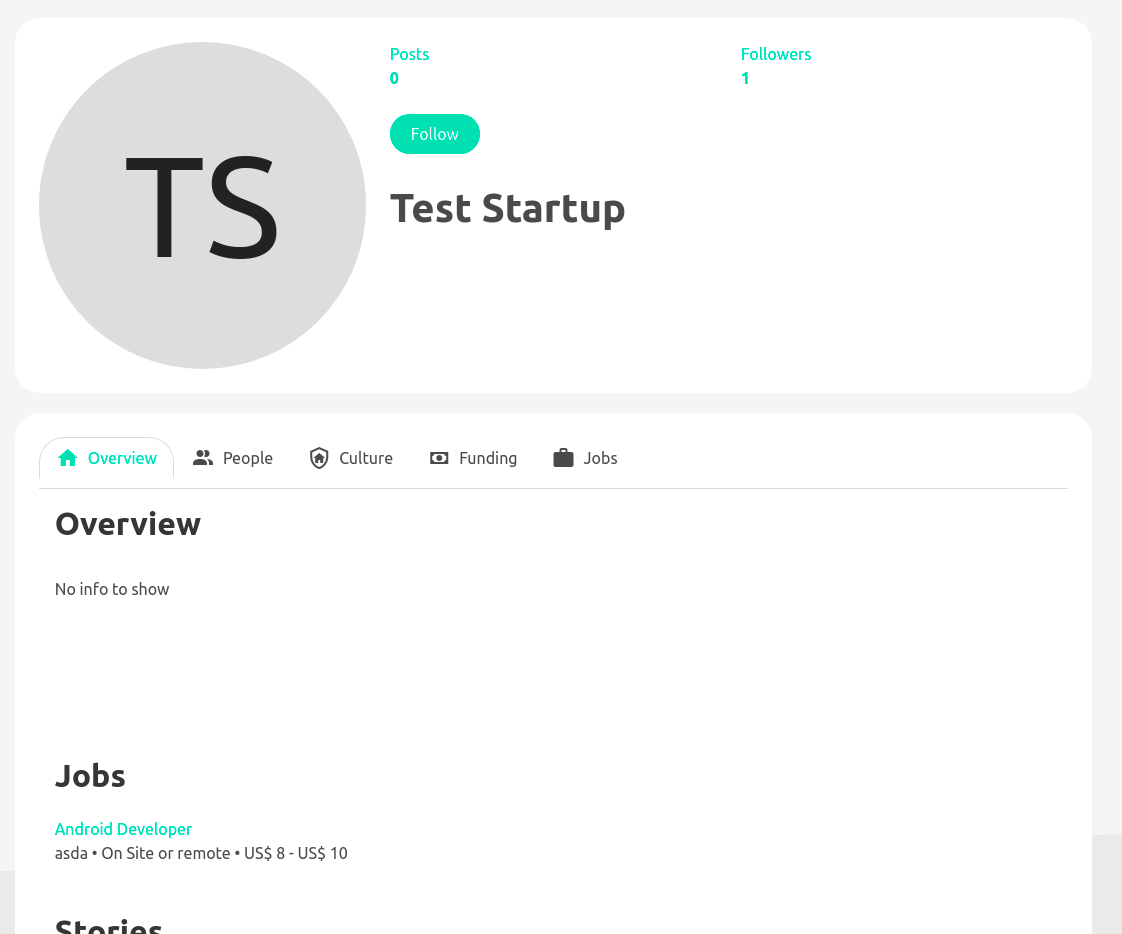
\includegraphics[width=0.60\textwidth]{img/53.png}
\caption{Perfil de una startup. Fuente: Propia}
\label{figure:startupProfileShow}
\end{figure}

\subsubsection{Listado de Productos}

En el listado de productos, por su parte, se ven los productos creados junto a su imagen, su nombre, su descripción básica, así como las etiquetas que lo describen. Así mismo, se tiene la posibilidad de votar al producto, para posicionarlo en la parte superior de la lista para los usuarios.

\begin{figure}[H]
\centering
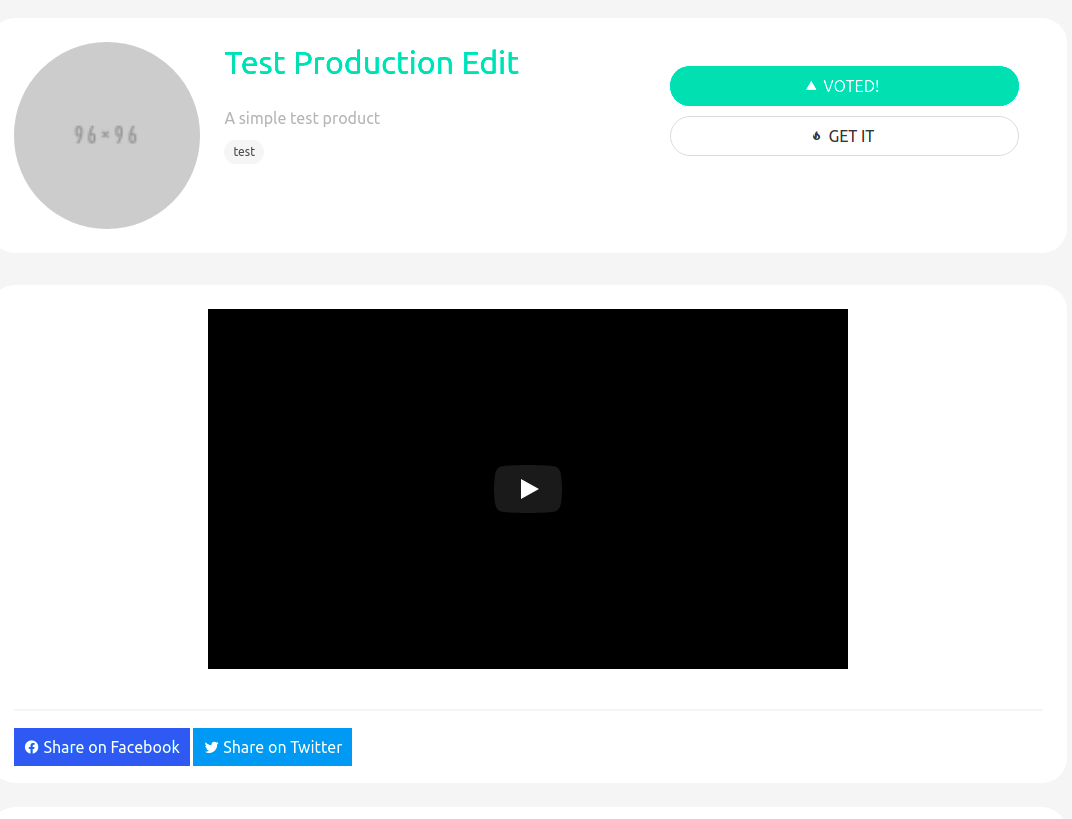
\includegraphics[width=0.60\textwidth]{img/54.png}
\caption{
Lista de Productos. Fuente: Propia}
\label{figure:productsList}
\end{figure}

Al acceder al perfil del producto, se puede ver toda la información introducida inicialmente para describir al mismo.

\begin{figure}[H]
\centering
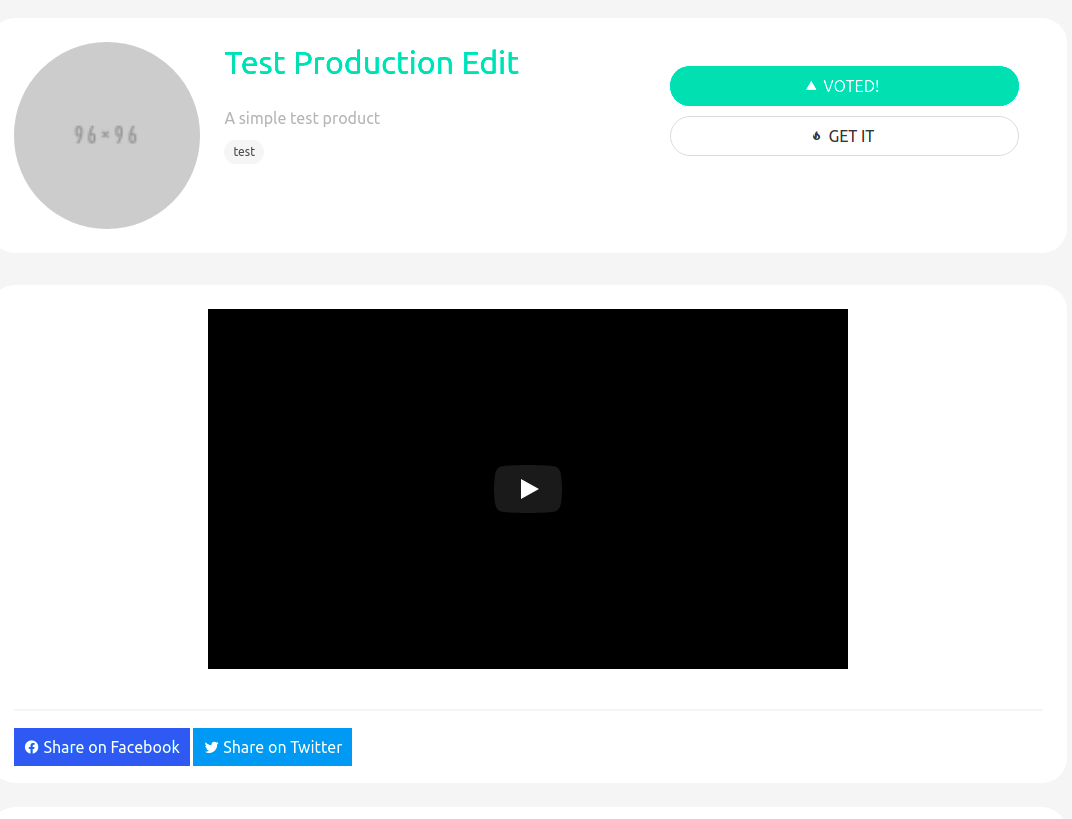
\includegraphics[width=0.60\textwidth]{img/55.png}
\caption{Perfil de producto. Fuente: Propia}
\label{figure:productProfileShow}
\end{figure}

El resto de las vistas (“Invitaciones”, “Inversores”, “Mentores”, “Asesores” y “Aliados”) al momento de finalizar este proyecto no habían sido implementadas por lo que únicamente se replicó el mismo formato que en el listado de startups.

